%pme2360
\section{Ex. 8.63}

% \begin{figure}[h]
% \begin{center}
% 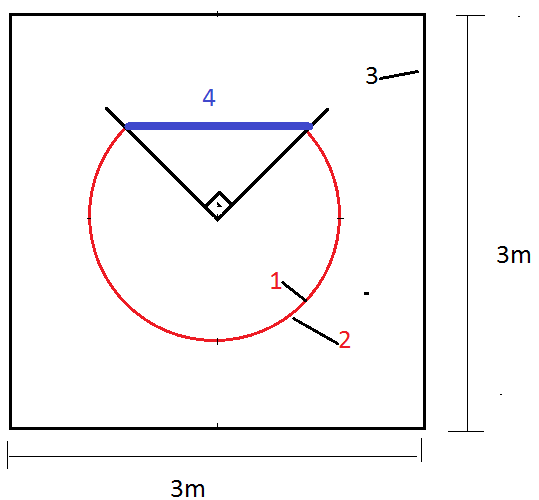
\includegraphics[scale=0.48]{./fig/1.png}
% \caption{\label{fig:1}fig 1} 
% \end{center}
% \end{figure}

\myfig[scale=.48]{figPME2360-20111019-01}{}

\begin{itemize}
\item $\rho$=900kg/m$^{3}$
\item $c_{0}$=200J/kgK
\item $\upsilon_{0}$=8.5*10$^{-4}$m$^{2}$/s
\item $k_{0}$=0.140 W/mK
\item $P_{R0}$=10$^{4}$ 
\end{itemize}

\paragraph*{Solução}

\[R_{eq}=\frac{1}{\bar{h} Pdx}+\frac{\ln(\frac{D_{0}}{D_{i}})}{2\pi dx k_{I}} \footnote{resistencia a conducao para uma parede cilindrica}+\frac{1}{sk_{s}}\]
s(tabela 4.1)-cilindro horizontal isotérmico de comprimento L enterrado em um meio semi-infinito

Para L $>>$ D
\[s'=\frac{2\pi L}{arccosh(\frac{2z}{D_{0}})}\]
\[s=s'\frac{dx}{L}\]
\[R_{eq}=\frac{1}{\bar{h} Pdx}+\frac{\ln(\frac{D_{0}}{D_{i}})}{2\pi dx k_{I}}+\frac{arccosh(\frac{2z}{D_{0}})}{2\pi dx k_{S}}\]

\[R_{eq}=\frac{R_{eq}'}{dx}\]
Balanço de energia

% \begin{figure}[h]
% \begin{center}
% 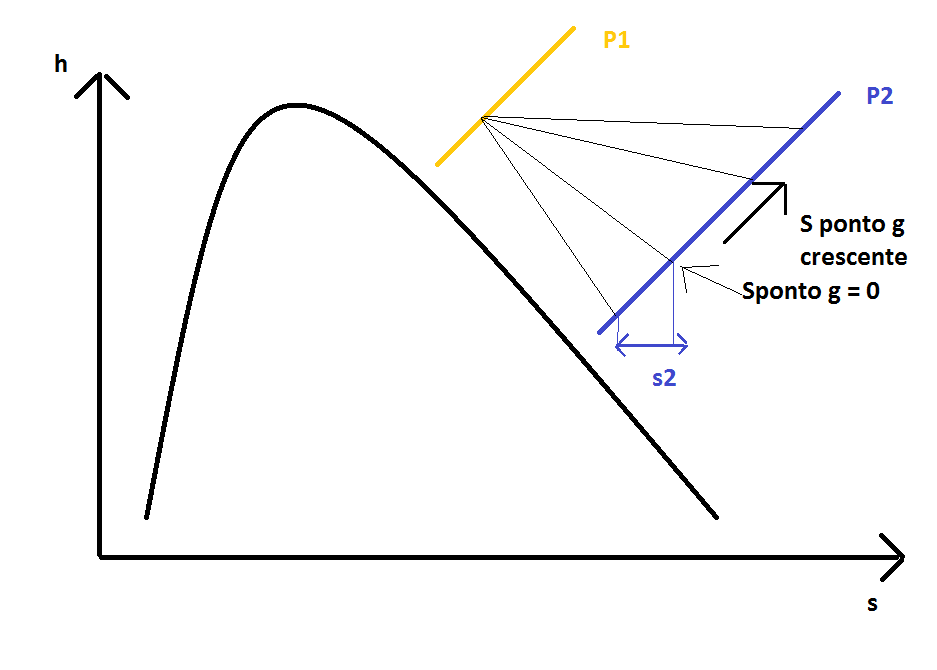
\includegraphics[scale=0.48]{./fig/2.png}
% \caption{\label{fig:1}fig 2} 
% \end{center}
% \end{figure}

\myfig[scale=.48]{figPME2360-20111019-02}{}

\[\dot{m}c_{0}T_{m}-\dot{m}c_{0}(T_{m}+dT_{m})+q''Pdx=0\]
\[\dot{m}c_{0}dT_{m}=q''Pdx\]
com:
\[q=\frac{Ts-Tm}{R_{eq}}\]
\[q''=\frac{Ts-Tm}{PdxR_{eq}}\]
\[\dot{m}cdT_{m}=\frac{T_{s}-T_{m}}{R'_{eq}}dx\]
\[dT_{m}=\frac{(T_{s}-T_{m})}{\dot{m}c_{0}R'_{eq}}dx\]

\[\theta = T_{s}-T_{m}\]
Portanto:
\[d\theta = -dT_{m}\]

\[d\theta = -\frac{\theta}{\dot{m}c_{0}R'_{eq}}dx\]

\[\int_{\theta _{e}}^{\theta _{s}}{\frac{d\theta}{\theta}}=\int_{x=0}^{x=L}{-\frac{dx}{\dot{m}c_{0}R'_{eq}}}\]

\begin{equation}
\frac{T_{m,s}-T_{s}}{T_{m,e}-T_{s}}=\exp(-\frac{L}{\dot{m}c_{0}R'_{eq}})
\label{eq:1}
\end{equation}


Cálculo de $\bar{h} $
\[
Re_{D}=\frac{\bar{\mu D_{i}}}{\upsilon _{0}}=\frac{\dot{m} D_{i}}{\upsilon _{0}\rho _{0} A_{tr}}\]
Onde $A_{tr}$=$\frac{\pi D_{i}^{2}}{4}$
\[\dot{m}=\rho _{0} \bar{\mu } A_{tr}\]
\[Re_{D}=\frac{4\dot{m}}{\upsilon _{0} \rho _{0} \pi D_{i}}=\frac{4*500}{8,5*10^{-4}*900*\pi * 1.2}=694\]

Como o resultado $<$ 2300, o regime é laminar

\[x_{CD,\upsilon}=0.05Re_{D}D\]
\[x_{CD,t}=x_{CD,\upsilon}*Pr\]

\[x_{CD,t}=4.16*10^{5}m\]

Estamos na região de entrada. Hausen $T_{sup}$ cte - interior do tubo.
\[\bar{Nu}_{D}=3.66+\frac{0.0668(\frac{D_{i}Re_{D}P_{R}}{L})}{1+0.04[\frac{D_{i}}{L}Re_{D}P_{R}]}=6.82\]

\[P_{r}>5\]
\[\bar{h}=\frac{Nu_{D}D_{I}}{k_{0}}=0.8W/m^{2}K\]

\[R_{eq}=\frac{1}{\bar{h} P}+\frac{\ln(\frac{D_{0}}{D_{i}})}{2\pi  k_{I}}+\frac{arccosh(\frac{2z}{D_{0}})}{2\pi  k_{S}}\]

\[R'_{eq}=0.33+0.71+0.66=1.7Km/W\]

\[\dot{q}=\dot{m}c_{0}(T_{m,e}-T_{m,s})=9.1*10^{6}W\]
Da equaçao \ref{eq:1}  $T_{m,s}$=111ºC

\section{8.60}  62 da 5a ed.

% \begin{figure}[h]
% \begin{center}
% 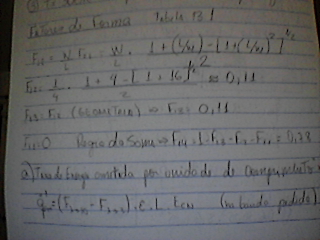
\includegraphics[scale=0.48]{./fig/3.png}
% \caption{\label{fig:1}fig 3} 
% \end{center}
% \end{figure}

\myfig[scale=.48]{figPME2360-20111019-03}{}

\begin{verbatim}
Entregar no dia da P2.
Tubo de parede delgada é usado pra transportar gases.
gas entra no tubo... ventos a uma temp de 15ºC em direcao
cruzada ao tubo a 5m/s. Considere as propriedades termofisicas
Estime coeficientes...

Temp media do fluido na saida -> balanço de volume de controle 
infinitesimal. Igual ao inicio do exercicio anterior. 
Temos 2 fluidos trocando energia entre quantas
resistencias em série? R: 3 (a de conveccao, a de conducao 
(parede do tubo) e a de conveeccao )
\end{verbatim}

\[R_{eq}=\frac{1}{h_{i}A_{i}} + cond\footnote{praticamente 0} + \frac{1}{h_{e}A_{e}}\]
Precisa verificar qual tipo de escoamento: no caso é turbulento.
Precisa verificar qual as regiões de entrada: 10 x o diametro. Tem 60 mm de comprimento.
A correlaçao que a gente usa é a Dittus- (Reynolds + Prandt)
Cálculo de $h_{i}$Eu avalio em qual temperatura? R: T média entre a entrada e a saída.
Deverá imaginar e chutar uma temperatura na saída. Avaliar as temperaturas médias e verificar o que resulta.

Cálculo de $h_{e}$:Kukauskas

\[Nu_{D}=cRe^{m}(\frac{Pr}{Pr_{S}})^{\frac{1}{4}}Pr^{n}\]

\[P_{R} \ de\  T _{\infty} \]

\[h_{i}(T_{m}-T_{s})=h_{e}(T_{S}-T_{\infty})\]